
\newgeometry{top=2.5cm, bottom=2.2cm, left=1.5cm, right=1.5cm}

\hypertarget{summaries}{\part{Résumés}}

{\normalfontsize

\vspace*{10pt}
\begin{minipage}[t]{.35\linewidth}

\paragraph{Structure du Tour}

\begin{tabular}{c|l}
1 & \hyperlink{movementphase}{Phase de Mouvement}. \tabularnewline
2 & \hyperlink{magicphase}{Phase de Magie}. \tabularnewline
3 & \hyperlink{shootingphase}{Phase de Tir}. \tabularnewline
4 & \hyperlink{closecombatphase}{Phase de Corps à Corps}. \tabularnewline
\end{tabular}

\vspace*{20pt}
\paragraph{Séquence Pré-Partie}

\begin{tabular}{c|l}
1 & Décidez de la \hyperlink{gamesize}{Taille de la Partie}. \tabularnewline
2 & \hyperlink{sharearmylist}{Montrez-vous vos Listes d'Armée}. \tabularnewline
3 & \hyperlink{buildbattlefield}{Installez le champ de bataille}. \tabularnewline
4 & Déterminez le \hyperlink{deploymenttype}{Type de Déploiement}. \tabularnewline
5 & Choisissez les \hyperlink{secondaryobjectives}{Objectifs Secondaires}. \tabularnewline
6 & Déterminez les \hyperlink{deploymentzones}{Zones de Déploiement}. \tabularnewline
7 & \hyperlink{generatespells}{Générez les Sorts}. \tabularnewline
8 & \hyperlink{deploymentphase}{Phase de Déploiement}. \tabularnewline
\end{tabular}

\vspace*{20pt}
\paragraph{Séquence de Déploiement}

\begin{tabular}{c|l}
1 & \hyperlink{whodeploysfirst}{Déterminez qui commence à se déployer}. \tabularnewline
2 & \hyperlink{deployunits}{Déployez des unités} chacun votre tour. \tabularnewline
3 & Déterminez qui veut jouer en premier. \tabularnewline
4 & \hyperlink{deployremainingunits}{Déployez les unités restantes}. \tabularnewline
5 & Déployez les \hyperlink{scout}{Éclaireurs}. \tabularnewline
6 & Déplacez les unités avec \hyperlink{vanguard}{\vanguard{}}. \tabularnewline
7 & Autres règles et capacités. \tabularnewline
8 & \hyperlink{rollforfirstturn}{Lancez le dé pour le premier tour}. \tabularnewline
\end{tabular}

\end{minipage}\hfill\begin{minipage}[t]{.60\linewidth}

\paragraph{Séquence de la Phase de Mouvement}

\begin{tabular}{c|p{9.6cm}}
1 & Début de la phase. \tabularnewline
2 & Début de l'étape des Charges. \tabularnewline
3 & Le Joueur Actif \hyperlink{declarecharges}{Déclare ses Charges}. Il nomme l'unité qui charge et sa cible. À chaque fois que le Joueur Actif déclare une charge, le Joueur Réactif doit annoncer et effectuer la \hyperlink{chargereaction}{Réaction à la Charge} de l'unité ciblée. \tabularnewline
4 & Une fois que toutes les charges et réactions ont été déclarées, les unités en charge tentent d'arriver au Corps à Corps : \hyperlink{movechargers}{le Joueur Actif effectue les jets de Distance de Charge}. \tabularnewline
5 & Si une unité en charge n'arrive pas à atteindre sa cible, elle doit faire un \hyperlink{failedchargemove}{Mouvement de Charge Ratée}. \tabularnewline
6 & Si une unité en charge a obtenu une distance suffisante pour atteindre sa cible, le Joueur Actif la déplace puis l'aligne en contact avec l'unité ciblée de manière à maximiser le contact. L'unité en charge et sa cible sont maintenant au Corps à Corps. \tabularnewline
7 & Fin de l'étape des Charges. \tabularnewline
8 & Début de l'étape des \hyperlink{compulsorymoves}{Mouvements Obligatoires}. \tabularnewline
9 & Le Joueur Actif peut essayer de rallier ses unités en fuite en passant des \hyperlink{rallytest}{Tests de Ralliement}. \tabularnewline
10 & Les unités toujours en fuite doivent effectuer un \hyperlink{fleemove}{Mouvement de Fuite}. \tabularnewline
11 & Les unités avec la règle \hyperlink{randommovement}{\randommovement{}} ou tout autre forme de mouvement obligatoire doivent maintenant se déplacer. \tabularnewline
12 & Fin de l'étape des Mouvements Obligatoires. \tabularnewline
13 & Début de l'étape des \hyperlink{remainingmoves}{Autres Mouvements}. \tabularnewline
14 & Les unités du Joueur Actif qui ne se sont pas encore déplacées pendant cette Phase de Mouvement peuvent maintenant effectuer un \hyperlink{advancemove}{Mouvement Simple}, une \hyperlink{marchmove}{Marche Forcée} ou une \hyperlink{reform}{Reformation}. \tabularnewline
15 & Fin de l'étape des Autres Mouvements. \tabularnewline
16 & Fin de la phase. \tabularnewline
\end{tabular}

\vspace*{20pt}
\begin{framed}
\paragraph{Terrains Dangereux}

Lancez le nombre de dés correspondant au Type de Troupe de la figurine.\newline
Terrain Dangereux (1) : le test rate sur un \result{1}.\newline
Terrain Dangereux (2) : le test rate sur \result{1} ou \result{2}.\newline
Terrain Dangereux (3) : le test rate sur \result{1}, \result{2} ou \result{3}.\newline
Une blessure avec la règle \armourpiercing{6} pour chaque test raté.
\end{framed}

\end{minipage}

\newpage

\begin{multicols}{2}\raggedcolumns

\paragraph{Séquence de la Phase de Magie}

\begin{tabular}{c|p{7.4cm}}
1 & Début de la Phase de Magie. Lancez les dés pour les \hyperlink{magicflux}{\textbf{Flux de Magie}} et la \hyperlink{magicflux}{\textbf{\channel}}. \tabularnewline
2 & Les sorts de type \hyperlink{remainsinplay}{\textbf{\remainsinplay}} peuvent être dissipés. \tabularnewline
3 & Le Joueur Actif peut \hyperlink{spellcastingsequence}{\textbf{tenter de lancer un sort}}. \tabularnewline
4 & Répétez les étapes 2 et 3 jusqu'à ce qu'aucun joueur ne tente quoi que ce soit. \tabularnewline
5 & Fin de la Phase de Magie. Les capacités prenant effet à la fin de la phase sont déclenchées. \tabularnewline
\end{tabular}

\vspace*{10pt}
\paragraph{Tentative de Lancement de Sort}

\begin{tabular}{c|m{7.4cm}}
1 & Le Joueur Actif indique quel Sorcier tente de lancer quel sort. Il doit préciser s'il opte pour une version améliorée du sort, ainsi que la cible du sort et de celle de l'attribut si nécessaire. Il indique enfin le nombre de Dés de Pouvoir utilisés, entre 1 et 5. \tabularnewline
2 & Le Joueur Actif lance le nombre de Dés de Pouvoir annoncé, en les retirant de sa réserve. Additionnez les résultats des dés avec les modificateurs magiques (tels qu'un Pouvoir Irrésistible) pour obtenir le total de lancement. \tabularnewline
3 & La tentative de lancement réussit si le total de lancement est \textbf{supérieur ou égal} à la valeur de lancement. Sinon, le lancement de sort échoue et le lanceur subit une \lostfocus{}. \tabularnewline
\end{tabular}

\vspace*{10pt}
\paragraph{Tentative de Dissipation}

\begin{tabular}{c|m{7.4cm}}
1 & Le Joueur Réactif peut désigner un Sorcier n'étant pas en fuite pour tenter la dissipation et annonce combien de Dés de Dissipation il va utiliser. Il doit utiliser au moins un dé et jusqu'à la totalité de sa réserve. Il est possible de tenter une dissipation même sans avoir de Sorcier. \tabularnewline
2 & Le Joueur Réactif lance le nombre de Dés de Dissipation annoncé, en les retirant de sa réserve. Additionnez les résultats des dés avec les modificateurs magiques (tels qu'un Pouvoir Irrésistible) pour obtenir le total de dissipation. \tabularnewline
3 & La tentative de dissipation réussit si le total de dissipation est \textbf{supérieur ou égal} au total de lancement. Le sort est alors dissipé et le lancement échoue. Sinon, la tentative de dissipation échoue et le Sorcier à l'origine de cette tentative subit une \lostfocus{}. \tabularnewline
\end{tabular}

\vspace*{20pt}
\begin{framed}
\vspace*{-17pt}
\paragraph{Modificateurs Magiques}

\noindent Sorcier Apprenti, Niveau 1 à 2 : +1

\vspace*{3pt}
\noindent Maître Sorcier, Niveau 3 à 4 : +2

\vspace*{3pt}
\noindent \overwhelmingpower{} : + 1D3 + NDU.

\vspace*{3pt}
\noindent La somme des modificateurs hors \overwhelmingpower{} ne peut pas dépasser +3.

\end{framed}

\vspace*{\fill}
\columnbreak

\paragraph{Table des \miscasts{}}

\begin{center}
\begin{tabular}{cm{6.75cm}@{}}
\hline
\textbf{2 à 4} & \textbf{\breachintheveil}

\vspace*{3pt}
Centrez le gabarit de \distance{5} sur le lanceur. Toute figurine touchée par le gabarit subit une touche.

\vspace*{3pt}
Si \textbf{4} Dés de Pouvoir ont été utilisés, lancez un dé. Sur un résultat de 1 à 3, retirez le lanceur de la partie.

\vspace*{3pt}
Si \textbf{5} Dés de Pouvoir ont été utilisés, retirez le lanceur de la partie.\tabularnewline
\textbf{5 à 6} & \textbf{\catastrophicdetonation}

\vspace*{3pt}
Centrez le gabarit de \distance{3} sur le lanceur. Toute figurine touchée par le gabarit subit une touche. Le lanceur doit subir une touche.\tabularnewline
\textbf{7} & \textbf{\witchfire}

\vspace*{3pt}
L'unité du lanceur subit NDU touches, distribuées comme des tirs. Le lanceur ne peut cependant subir qu'une seule touche au plus.\tabularnewline
\textbf{8 à 9} & \textbf{\sorcerousbacklash}

\vspace*{3pt}
Le lanceur et tout Sorcier allié subissent une touche. \tabularnewline
\textbf{10 à 12} & \textbf{\amnesia}

\vspace*{3pt}
Le Niveau de Magie du lanceur est diminué de NDU-2. Il perd un sort pour chaque Niveau de Magie perdu, en commençant par le sort ayant causé le \miscast{} et en tirant les autres au hasard.\tabularnewline
\hline
\end{tabular}
\end{center}

\vspace*{5pt}
\noindent Les touches infligées par un \miscast{} ont une Force de NDU+2 et les règles \magicalattacks{} et \armourpiercing{1}. Le Sorcier ayant provoqué le \miscast{} ne peut utiliser aucune sauvegarde.

\vspace*{5pt}
\noindent Quel que soit le résultat du jet, retirez NDU Dés de Pouvoir de la réserve du propriétaire du lanceur.

\vspace*{30pt}
\begin{framed}
\vspace*{-17pt}
\paragraph{\boundspells{}}

\noindent Pour lancer un sort lié à un Objet de Sort avec succès, le jet de lancement doit être supérieur ou égal à son Niveau de Puissance.
\begin{itemize}[label={-}]
\item Aucun modificateur positif ne peut être ajouté au jet de lancement.
\item Un échec ne provoque pas de \lostfocus{} pour le lanceur.
\item Un objet de sort ne bénéficie pas du bonus de lancement d'un Pouvoir Irrésistible.
\item L'Attribut de la Voie est lancé normalement.
\end{itemize}

\noindent En cas de Pouvoir Irrésistible :
\begin{itemize}[label={-}, itemsep=3pt]
\item Si 4 dés ou plus ont été lancés, l'\boundspell{} est perdu et le sort ne peut plus être lancé de la partie.
\item Retirez NDU Dés de Pouvoir de la réserve du propriétaire du lanceur.
\end{itemize}
\end{framed}

\vspace*{\fill}
\end{multicols}

\newpage

\begin{minipage}[t]{.68\linewidth}

\paragraph{Phase de Tir}

\begin{tabular}{c|p{11cm}}
1 & Le Joueur Actif peut choisir une unité autorisée à effectuer une Attaque de Tir et déclarer la cible. \tabularnewline
2 & Le Joueur Actif doit \hyperlink{measuringdistances}{Mesurer la Distance} pour s'assurer que l'unité ennemie ciblée est bien à portée de l'Attaque de Tir. Il doit aussi vérifier que la cible est en \hyperlink{lineofsight}{Ligne de Vue}. \tabularnewline
3 & Le Joueur Actif effectue les jets pour toucher et compare avec la Table pour toucher au Tir. \tabularnewline
4 & Il fait un \hyperlink{towoundroll}{Jet pour Blesser} pour chaque touche réussie. \tabularnewline
5 & Pour chaque blessure reçue, le Joueur Réactif peut tenter une \hyperlink{armoursaveandmodifiers}{Sauvegarde d'Armure} et une \hyperlink{regeneration}{Sauvegarde de \regeneration{}} ou une \hyperlink{wardsave}{\wardsave{}} selon les possibilités de la figurine blessée. \tabularnewline
6 & Le Joueur Réactif \hyperlink{removecasualties}{Retire les Pertes} pour chaque blessure non sauvegardée et marque les blessures infligées aux figurines à plusieurs PVs. \tabularnewline
7 & Le Joueur Actif peut sélectionner une nouvelle unité pour tirer et retourner à l'étape 1. \tabularnewline
8 & Dès qu'une unité atteint de Lourdes Pertes, c'est-à-dire dès qu'elle a perdu au moins 25\% de ses effectifs pendant la Phase de Tir, elle doit passer un \hyperlink{panictest}{Test de Panique}. \tabularnewline
9 & Fin de la phase. \tabularnewline
\end{tabular}

\vspace*{10pt}
\paragraph{Table des Incidents de Tir}

\begin{center}
\begin{tabular}{M{2cm}m{8cm}}
\textbf{Résultat} & \centering\textbf{Effet} \tabularnewline
\hline
\textbf{0 ou moins} & \textbf{Explosion !}\vspace*{3pt}\newline 
Toutes les figurines à moins de \distance{1D6} de l'Arme d'Artillerie subissent une touche de Force 5. L'Arme d'Artillerie est détruite, retirez-la comme perte. \tabularnewline
\textbf{1 à 2} & \textbf{Défaillance Critique}\vspace*{3pt}\newline 
Le mécanisme de tir est endommagé. La figurine ne peut plus tirer avec cette arme pour le restant de la partie. \tabularnewline
\textbf{3 à 4} & \textbf{Enrayé}\vspace*{3pt}\newline
Cette Arme d'Artillerie ne peut pas être utilisée au prochain Tour de Joueur du propriétaire. \tabularnewline
\textbf{5+} & \textbf{Dysfonctionnement}\vspace*{3pt}\newline
La figurine subit une blessure sans sauvegarde d'aucune sorte possible. \tabularnewline
\hline
\end{tabular}
\end{center}

\end{minipage}\hfill\begin{minipage}[t]{.29\linewidth}

\paragraph{Table pour toucher au Tir}

\begin{center}
\begin{tabular}{rl}
\hline
\textbf{CT + Modif.} & \textbf{Résultat nécessaire} \tabularnewline
6 ou plus & 2+ \tabularnewline
5 & 2+ \tabularnewline
4 & 3+ \tabularnewline
3 & 4+ \tabularnewline
2 & 5+ \tabularnewline
1 & \result{6} \tabularnewline
0 & \result{6} suivi d'un 4+ \tabularnewline
-1 & \result{6} suivi d'un 5+ \tabularnewline
-2 & \result{6} suivi d'un \result{6} \tabularnewline
-3 ou moins & impossible \tabularnewline
\hline
\end{tabular}
\end{center}

\vspace*{10pt}
\paragraph{Pénalités pour toucher}

\begin{center}
\begin{tabular}{rl}
\hline
Bouger et Tirer & -1 \tabularnewline
Longue Portée & -1 \tabularnewline
Tenir la Position et Tirer & -1 \tabularnewline
Couvert Léger & -1 \tabularnewline
Couvert Lourd & -2 \tabularnewline
\hline
\end{tabular}
\end{center}

\end{minipage}

\vspace*{20pt}
\def\svgwidth{\textwidth}
\input{pics/line_of_sight_and_cover_summary.pdf_tex}

\newpage

\begin{multicols}{2}\raggedcolumns

\paragraph{Phase de Corps à Corps}

\begin{tabular}{c|p{7.4cm}}
1 & Début de la Phase de Corps à Corps. Appliquez la règle \hyperlink{nolongerengaged}{Plus Engagés} si nécessaire. \tabularnewline
2 & Le Joueur Actif choisit un combat. \tabularnewline
3 & Résolvez cette Manche de Corps à Corps. \tabularnewline
4 & Répétez les étapes 2 et 3 pour chaque combat qui n'a pas encore eu lieu pendant cette phase. \tabularnewline
5 & Une fois que toutes les unités engagées au Corps à Corps ont combattu, la Phase de Corps à Corps prend fin. \tabularnewline
\end{tabular}

\paragraph{Séquence d'une Manche de Corps à Corps}

\begin{tabular}{c|p{7.3cm}}
1 & Début de la Manche de Corps à Corps. \tabularnewline
2 & Choisissez les armes. \tabularnewline
3 & Appliquez la règle \hyperlink{makeway}{Faites Place}. \tabularnewline
4 & Lancez et relevez ou refusez les \hyperlink{challenges}{Défis}. \tabularnewline
5 & Exécutez les attaques par palier d'Initiative :
	\begin{enumerate}[parsep=0cm,itemsep=0.05cm, topsep=3pt]
		\item Allouez les attaques.
		\item Lancez les jets pour toucher, pour blesser, les jets de sauvegarde et retirez les pertes.
		\item Recommencez pour le palier d'Initiative suivant.
 	\end{enumerate}\tabularnewline
6 & Déterminez quel camp a gagné cette Manche de Corps à Corps. Le(s) perdant(s) passent un \hyperlink{breaktest}{Test de Moral}. \tabularnewline
7 & En cas d'échec, les unités alliées à moins de \distance{6} passent un \hyperlink{panictest}{Test de Panique}. \tabularnewline
8 & En cas de fuite, choisissez de poursuivre ou de vous réfréner. \tabularnewline
9 & Jet des distances de fuite. \tabularnewline
10 & Jet des distances de poursuite. \tabularnewline
11 & Déplacement des unités en fuite. \tabularnewline
12 & Déplacement des unités poursuivantes. \tabularnewline
13 & \hyperlink{postcombatpivots}{Pivots Post-Combat ou Reformations Post-Combat}. \tabularnewline
14 & \hyperlink{combatreform}{Reformations de Combat}. \tabularnewline
15 & Fin de la manche, passez au prochain Corps à Corps. \tabularnewline
\end{tabular}

\paragraph{Quand une attaque touche}

\begin{tabular}{c|p{7.4cm}}
1 & L'Attaquant \hyperlink{distributehits}{Répartit les touches}. \tabularnewline
2 & L'Attaquant lance les jets pour blesser. Passez à l'étape suivante pour les jets réussis. \tabularnewline
3 & Le Défenseur tente ses Sauvegardes d'Armure. Passez à l'étape suivante pour les jets ratés. \tabularnewline
4 & Le Défenseur tente ses sauvegardes spéciales. Passez à l'étape suivante pour les jets ratés. \tabularnewline
5 & Le Défenseur retire les PVs et les pertes. \tabularnewline
6 & Le Défenseur passe éventuellement un \hyperlink{panictest}{Test de Panique}. \tabularnewline
\end{tabular}

\paragraph{Modificateur d'Armure}

\begin{center}
\begin{tabular}{c@{\hspace{0.5cm}}cccccccccc}
\hline
\textbf{Force} & \textbf{1} & \textbf{2} & \textbf{3} & \textbf{4} & \textbf{5} & \textbf{6} & \textbf{7} & \textbf{8} & \textbf{9} & \textbf{10} \tabularnewline
\textbf{Malus} & 0 & 0 & 0 & \red -1 & \red -2 & \red -3 & \red -4 & \red -5 & \red -6 & \red -6 \tabularnewline
\hline
\end{tabular}
\end{center}

\vspace*{\fill}
\columnbreak

\paragraph{Résumé du Résultat de Combat}

\begin{center}
\begin{tabular}{rl}
\hline
Blessures Infligées & \textbf{+1} par blessure \tabularnewline
Massacre & \textbf{+1} par blessure (max. \textbf{+3}) \tabularnewline
Charge & \textbf{+1} (\textbf{+2} depuis une Colline) \tabularnewline
Bonus de Rang & \textbf{+1} par rang (max. \textbf{+3}) \tabularnewline
Porte-Étendard & \textbf{+1} \tabularnewline
Grande Bannière & \textbf{+1} \tabularnewline
Attaque de Flanc & \textbf{+1} ou \textbf{+2} \tabularnewline
Attaque de l'Arrière & \textbf{+2} ou \textbf{+3} \tabularnewline
\hline
\end{tabular}
\end{center}

\vspace*{10pt}
\begin{framed}
\vspace*{-17pt}
\paragraph{Général et Porteur de la Grande Bannière}

\begin{itemize}[label={-}]
\item Un Général non en fuite donne son Commandement à toutes les unités alliées à moins de \distance{12}.
\item Un Porteur de la Grande Bannière non en fuite donne la capacité de relancer leurs tests de Commandement ratés à toutes les unités alliées à moins de \distance{12}.
\item Une \largetarget{} augmente la portée des deux règles précédentes de \distance{6}.
\end{itemize}
\end{framed}

\paragraph{Table pour toucher au Corps à Corps}

\begin{center}
\begin{tabular}{c|cccccccccc@{}}
\backslashbox{\textbf{D}}{\textbf{A}} & \textbf{1} & \textbf{2} & \textbf{3} & \textbf{4} & \textbf{5} & \textbf{6} & \textbf{7} & \textbf{8} & \textbf{9} & \textbf{10} \\
\hline
\textbf{1} & \yel 4+ & \lem 3+ & \lem 3+ & \lem 3+ & \lem 3+ & \lem 3+ & \lem 3+ & \lem 3+ & \lem 3+ & \lem 3+ \\
\textbf{2} & \yel 4+ & \yel 4+ & \lem 3+ & \lem 3+ & \lem 3+ & \lem 3+ & \lem 3+ & \lem 3+ & \lem 3+ & \lem 3+ \\
\textbf{3} & \ora 5+ & \yel 4+ & \yel 4+ & \lem 3+ & \lem 3+ & \lem 3+ & \lem 3+ & \lem 3+ & \lem 3+ & \lem 3+ \\
\textbf{4} & \ora 5+ & \yel 4+ & \yel 4+ & \yel 4+ & \lem 3+ & \lem 3+ & \lem 3+ & \lem 3+ & \lem 3+ & \lem 3+ \\
\textbf{5} & \ora 5+ & \ora 5+ & \yel 4+ & \yel 4+ & \yel 4+ & \lem 3+ & \lem 3+ & \lem 3+ & \lem 3+ & \lem 3+ \\
\textbf{6} & \ora 5+ & \ora 5+ & \yel 4+ & \yel 4+ & \yel 4+ & \yel 4+ & \lem 3+ & \lem 3+ & \lem 3+ & \lem 3+ \\
\textbf{7} & \ora 5+ & \ora 5+ & \ora 5+ & \yel 4+ & \yel 4+ & \yel 4+ & \yel 4+ & \lem 3+ & \lem 3+ & \lem 3+ \\
\textbf{8} & \ora 5+ & \ora 5+ & \ora 5+ & \yel 4+ & \yel 4+ & \yel 4+ & \yel 4+ & \yel 4+ & \lem 3+ & \lem 3+ \\
\textbf{9} & \ora 5+ & \ora 5+ & \ora 5+ & \ora 5+ & \yel 4+ & \yel 4+ & \yel 4+ & \yel 4+ & \yel 4+ & \lem 3+ \\
\textbf{10} & \ora 5+ & \ora 5+ & \ora 5+ & \ora 5+ & \yel 4+ & \yel 4+ & \yel 4+ & \yel 4+ & \yel 4+ & \yel 4+ \\
\end{tabular}
\end{center}

\paragraph{Table pour blesser}

\begin{center}
\begin{tabular}{c|cccccccccc@{}}
\backslashbox{\textbf{E}}{\textbf{F}} & \textbf{1} & \textbf{2} & \textbf{3} & \textbf{4} & \textbf{5} & \textbf{6} & \textbf{7} & \textbf{8} & \textbf{9} & \textbf{10} \tabularnewline
\hline
\textbf{1} & \yel 4+ & \lem 3+ & \gre 2+ & \gre 2+ & \gre 2+ & \gre 2+ & \gre 2+ & \gre 2+ & \gre 2+ & \gre 2+ \tabularnewline
\textbf{2} & \ora 5+ & \yel 4+ & \lem 3+ & \gre 2+ & \gre 2+ & \gre 2+ & \gre 2+ & \gre 2+ & \gre 2+ & \gre 2+ \tabularnewline
\textbf{3} & \red 6+ & \ora 5+ & \yel 4+ & \lem 3+ & \gre 2+ & \gre 2+ & \gre 2+ & \gre 2+ & \gre 2+ & \gre 2+ \tabularnewline
\textbf{4} & \red 6+ & \red 6+ & \ora 5+ & \yel 4+ & \lem 3+ & \gre 2+ & \gre 2+ & \gre 2+ & \gre 2+ & \gre 2+ \tabularnewline
\textbf{5} & \red 6+ & \red 6+ & \red 6+ & \ora 5+ & \yel 4+ & \lem 3+ & \gre 2+ & \gre 2+ & \gre 2+ & \gre 2+ \tabularnewline
\textbf{6} & \red 6+ & \red 6+ & \red 6+ & \red 6+ & \ora 5+ & \yel 4+ & \lem 3+ & \gre 2+ & \gre 2+ & \gre 2+ \tabularnewline
\textbf{7} & \red 6+ & \red 6+ & \red 6+ & \red 6+ & \red 6+ & \ora 5+ & \yel 4+ & \lem 3+ & \gre 2+ & \gre 2+ \tabularnewline
\textbf{8} & \red 6+ & \red 6+ & \red 6+ & \red 6+ & \red 6+ & \red 6+ & \ora 5+ & \yel 4+ & \lem 3+ & \gre 2+ \tabularnewline
\textbf{9} & \red 6+ & \red 6+ & \red 6+ & \red 6+ & \red 6+ & \red 6+ & \red 6+ & \ora 5+ & \yel 4+ & \lem 3+ \tabularnewline
\textbf{10} & \red 6+ & \red 6+ & \red 6+ & \red 6+ & \red 6+ & \red 6+ & \red 6+ & \red 6+ & \ora 5+ & \yel 4+ \tabularnewline
\end{tabular}
\end{center}

\vspace*{\fill}
\end{multicols}

\newpage

\paragraph{Résumé des Types de Troupe}

\rowcolors{1}{white}{black!10}
\begin{center}
\begin{tabular}{@{}>{\bfseries}M{2.5cm}M{2cm}M{2.2cm}M{2.2cm}M{3cm}M{1.8cm}M{1.3cm}@{}}
 & \textbf{Type de Profil} & \textbf{Rang Complet (Horde)} & \textbf{Soutien} & \textbf{Règles Spéciales} & \textbf{Taille$^{2}$} & \textbf{DTD$^{3}$} \tabularnewline
\infantry{} & - & 5 (10) & 1 & - & Petite & 1 \tabularnewline

\warbeast{} & - & 5 (10) & 1 & \swiftstride{} & Petite & 1 \tabularnewline

\cavalry{} & \combinedprofile{} & 5 (10) & 1 (cavalier uniquement) & \swiftstride{} & Moyenne & 1 \tabularnewline

\monstrousinfantry{} & - & 3 (6) & jusqu'à 3 & \stomp{1} & Moyenne & 2 \tabularnewline

\monstrousbeast{} & - & 3 (6) & jusqu'à 3 & \swiftstride{}\newline \stomp{1} & Moyenne & 2 \tabularnewline

\monstrouscavalry{} & \combinedprofile{} & 3 (6) & jusqu'à 3 (cavalier uniquement) & \swiftstride{}\newline \stomp{1} & Moyenne & 2 \tabularnewline

\chariot{} & \combinedprofile{} & 3 (6) & 1 (1 membre d'équipage uniquement) & \swiftstride{} \newline \cannotmarch{} \newline \impacthits{1D6} & Moyenne & 4 \tabularnewline

\monster{} & - & 1 & - & \largetarget{} \newline \stomp{1D6} \newline \terror{} & Grande & 4 \tabularnewline

\riddenmonster{} & Profil de Monstre Monté & 1 & - & \largetarget{} \newline \stomp{1D6} \newline \terror{} & Grande & 4 \tabularnewline

\swarm{} & - & $^{1}$ (10) & 1 & \unbreakable{} \newline \unstable{} \newline \skirmisher{} & Petite & 1 \tabularnewline

\warmachine{} & Profil de Machine de Guerre & Pas de rangs & - & \moveorfire{} \newline \cannotmarch{} \newline \reload{} & Petite & 1 \tabularnewline
\end{tabular}
\end{center}
\noindent $^{1}$ Les Nuées ne peuvent pas avoir de Rang Complet puisqu'elles ont la règle \skirmisher{}.\newline
\noindent $^{2}$ Une figurine avec la règle \largetarget{} est de Grande Taille.\newline
\noindent $^{3}$ DTD : Dés utilisés pour les tests de Terrain Dangereux.

\paragraph{Décors Particuliers}

\noindent TD : Terrain Dangereux. CCCM : Cavalerie, Chars et Cavalerie Monstrueuse.

\rowcolors{1}{white}{black!10}
\begin{center}
\begin{tabular}{@{}>{\bfseries}M{2cm}M{4.8cm}M{4.8cm}M{4.8cm}}
\textbf{Décor} & \textbf{Mouvement} & \textbf{Couvert} & \textbf{Autres} \tabularnewline
\hyperlink{fields}{Champ} &
TD (1) pour CCCM et figurines avec \flamingattacks{}. &
Offre un Couvert Léger si au moins de la moitié de l'Empreinte au Sol est dans le Champ. Ne s'applique pas à une \largetarget{}. &
Donne \flammable{}. \tabularnewline
\hyperlink{hills}{Colline} &
- &
Décor Occultant.\newline
Partiellement sur la Colline : Couvert Léger.\newline
Complétement hors de la Colline : Couvert Lourd.&
Donne \largetarget{}.\newline
Charger depuis la Colline donne +1 au Résultat de Combat. \tabularnewline
\hyperlink{water}{\water} &
TD (1) pour CCCM. &
- &
Supprime les Rangs Complets.\tabularnewline
\hyperlink{forests}{Forêt} &
TD (1) pour CCCM et les unités effectuant un Mouvement de \fly{}. &
Offre un Couvert Léger. &
Supprime Indomptable. Donne \stubborn{} aux \skirmishers{} et aux Personnages d'Infanterie seuls.\tabularnewline
\hyperlink{walls}{Mur} &
Ignorer le Mur pour le déplacement et le positionnement. TD (1) pour CCCM. &
Offre un Couvert Lourd. \distracting{} à la première Manche de Corps à Corps. Ne s'applique pas à une \largetarget{}. &
- \tabularnewline
\hyperlink{ruins}{Ruines} &
TD (1) pour toute unité non \skirmisher{}. TD(2) pour CCCM. &
Partiellement dans les Ruines : Couvert Lourd. Ne s'applique pas à une \largetarget{}. &
- \tabularnewline
\hyperlink{impassableterrain}{Terrain Infranchissable} &
\distance{1} d'écart.\newline
TD (3) pour les unités en fuite. &
Décor Occultant\newline
Couvert Lourd &
- \tabularnewline
\end{tabular}
\end{center}

\newpage

\paragraph{Touches de Gabarit}

Placement optimal des Gabarits circulaires. Les socles verts font \unit{20x20}{\milli\meter}, les socles magenta \unit{25x25}{\milli\meter}, les socles cyan \unit{40x40}{\milli\meter} et les socles oranges \unit{25x50}{\milli\meter}.

\vspace*{10pt}

{\largefontsize
\def\svgwidth{\textwidth}
\input{pics/Templates.pdf_tex}}

\vspace*{10pt}

\begin{center}
\begin{tabular}{M{2.5cm}M{2.5cm}M{2.5cm}M{2.5cm}M{2.5cm}}
\hline
Taille de socle & \unit{20x20}{\milli\meter} & \unit{25x25}{\milli\meter} & \unit{40x40}{\milli\meter} & \unit{25x50}{\milli\meter} \tabularnewline
Gabarit de \distance{3} & 22 & 16 & 9 & 11 \tabularnewline
Gabarit de \distance{5} & 48 & 34 & 16 & 24 \tabularnewline
\hline
\end{tabular}
\end{center}

\vspace*{20pt}

Un \linetemplate{} est une ligne droite tracée entre deux points. \newfromWHB{Toutes les figurines dont le socle se situe sous la ligne sont touchées.} On peut aussi déterminer le nombre de figurines touchées en additionnant le nombre de rangs et de colonnes traversés et en retirant un. Dans la figure \ref{figure/linetemplate}, 4 rangs et 4 colonnes sont traversés, soit 4 + 4 - 1 = 7 figurines touchées.

\vspace*{10pt}

\begin{center}
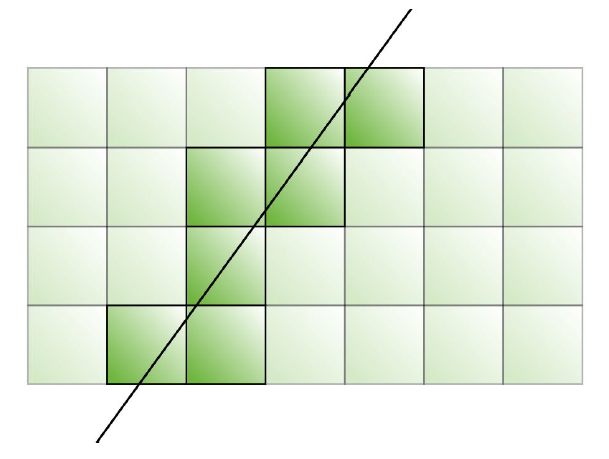
\includegraphics[width=7cm]{pics/linetemplate.png}
\end{center}
}